\documentclass[../../paper.tex]{subfiles}
\begin{document}
\section{Appendix}
\subsection{Journal Plots}
We created four seperate journal plots, Figures~\ref{figure:titlePlotNormal} and~\ref{figure:titlePlotGrouped} show the title based embeddings, and Figures~\ref{figure:abstractPlotNormal} and~\ref{figure:abstractPlotGrouped} show the abstract based embeddings.
Figures~\ref{figure:titlePlotNormal} and~\ref{figure:abstractPlotNormal} show the two dimensional plots of the journal embeddings. The journals are color-marked by publisher. Red is Wiley, lime is Elsevier and blue is Springer Nature. The grey points are other or not-specified publishers.
Figures~\ref{figure:titlePlotGrouped} and~\ref{figure:abstractPlotGrouped} show the journal embeddings grouped by a k-means algorithm, creating 8 groups. The bottom right of the plot shows the names of the journals closest to the center of the group. While most names state the topic of the research field, two do not. These are \textit{RSC Advances}: chemical sciences, and \textit{Symmetry}:  research on symmetry phenomena wherever they occur in mathematical or scientific studies. The k-means algorithm ran on the 300-dimensional vectors, while the plot shows the 2-dimensional vectors. In the title-based Figures (\ref{figure:titlePlotNormal} \&~\ref{figure:titlePlotGrouped}) the journals \textit{PNAS} and \textit{Cell} overlap each others labels on the bottom right side of the graph. In the abstract-based Figures (\ref{figure:abstractPlotNormal} \&~\ref{figure:abstractPlotGrouped}) the journals \textit{PNAS} and \textit{Nature} overlap each others label on the bottom right side of the graph.
The digital versions of these plots can be found at:~\url{https://goo.gl/nCGMcu} (title-based) and~\url{https://goo.gl/LwYP6k} (abstract-based). The usage of this digital version is advised, since this interactive plot enables zooming and adjusting plot settings, which can give a broader insight into the results than the presented figures. Although the presented figures give sufficient insight for the purpose of this thesis.
\begin{landscape}
\begin{figure}
\begin{center}
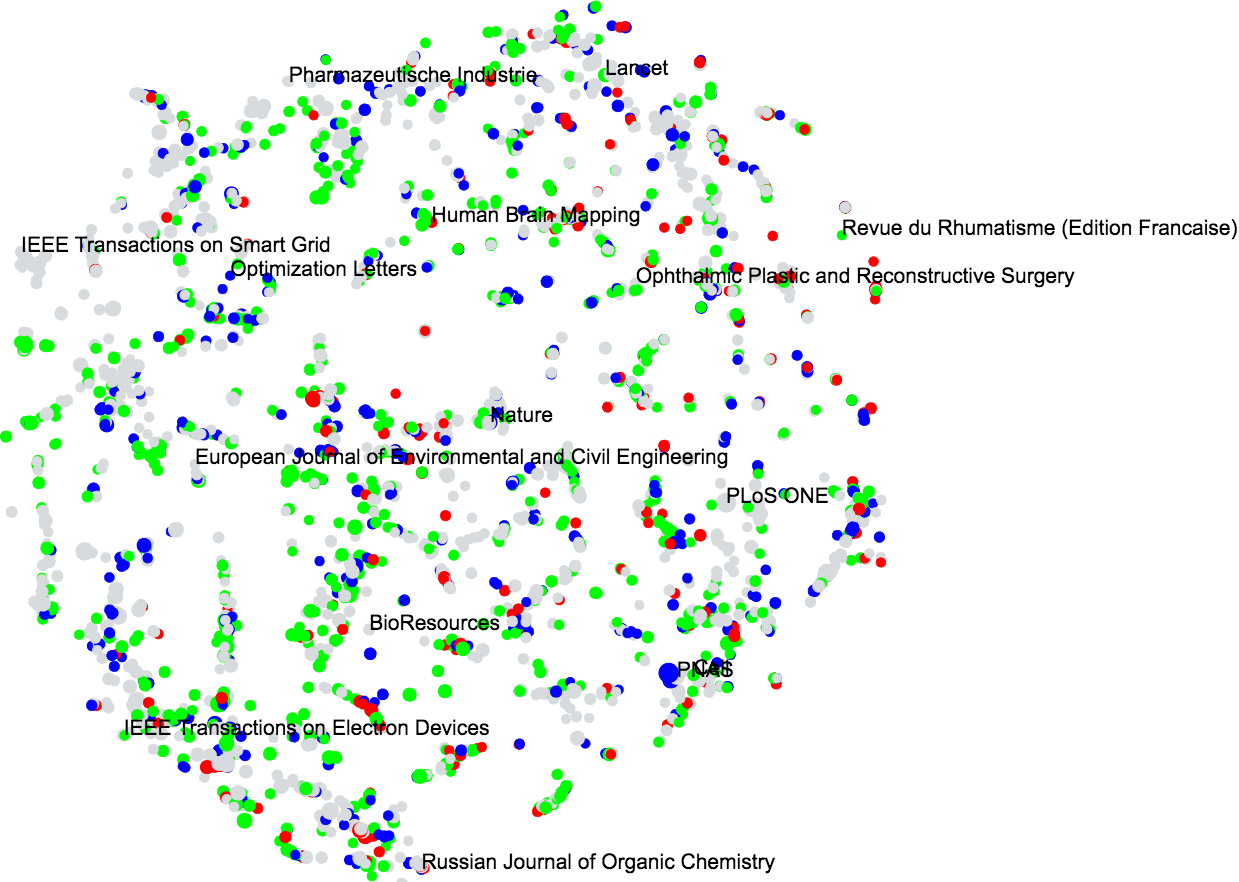
\includegraphics[height=6.5in]{Plots/Journal_Plots/Title_normal}
\end{center}
\caption{Journal plot of title embeddings, grouped by publisher}\label{figure:titlePlotNormal}
\end{figure}
\end{landscape}

\begin{landscape}
\begin{figure}
\begin{center}
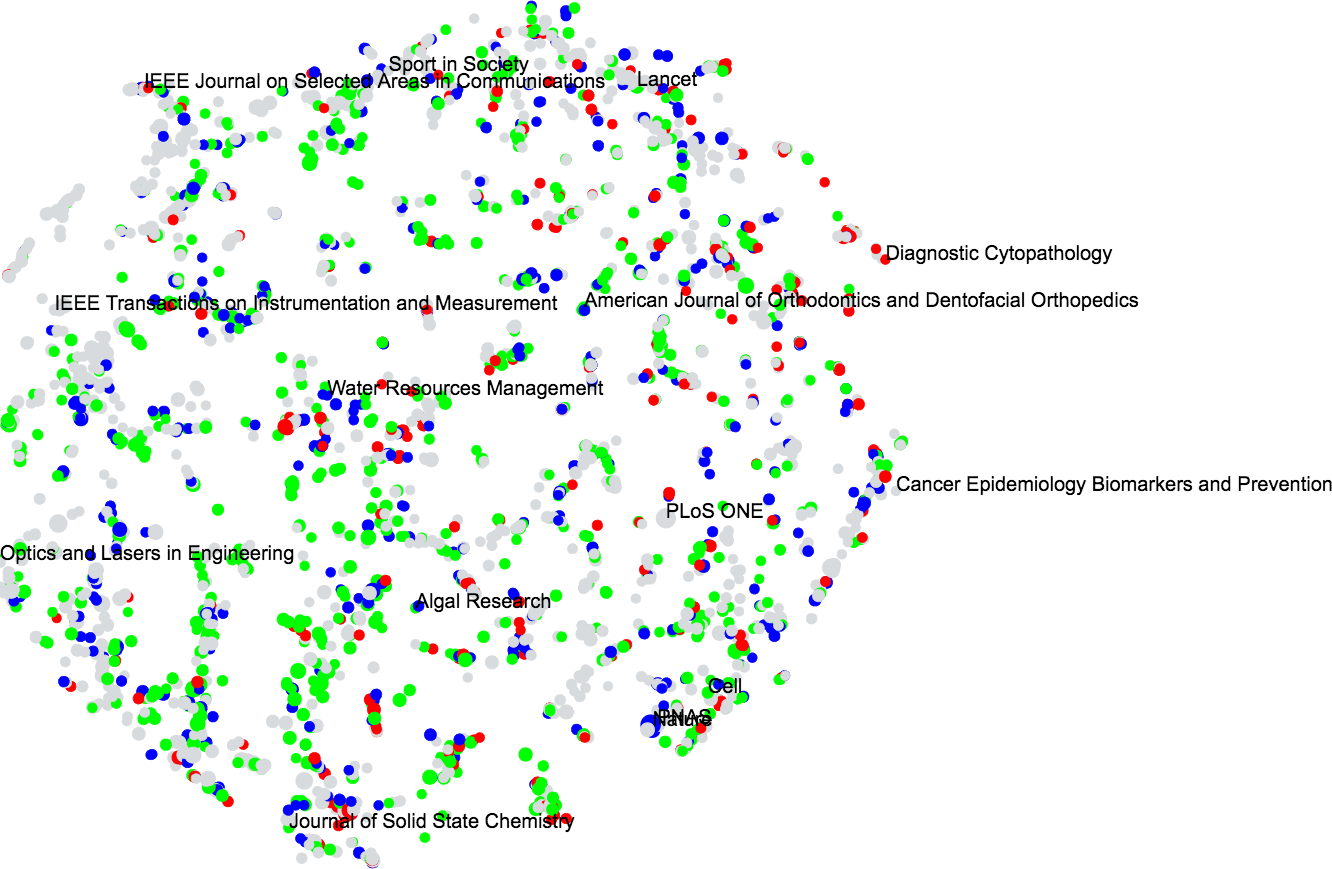
\includegraphics[height=6.5in]{Plots/Journal_Plots/Abstract_normal}
\end{center}
\caption{Journal plot of abstract embeddings, grouped by publisher}\label{figure:abstractPlotNormal}
\end{figure}
\end{landscape}

\begin{landscape}
\begin{figure}
\begin{center}
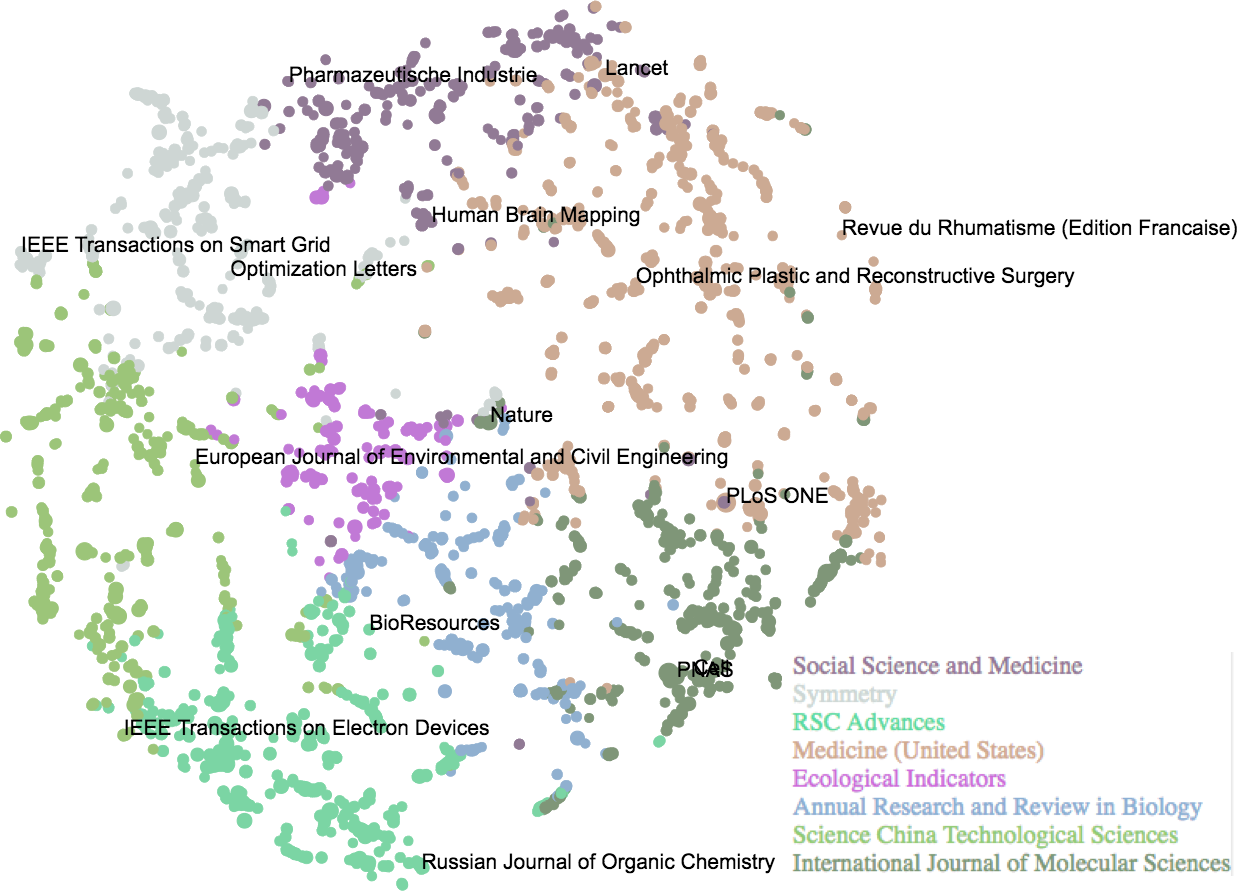
\includegraphics[height=6.5in]{Plots/Journal_Plots/Title_grouped}
\end{center}
\caption{Journal plot of title embeddings, k-means grouped}\label{figure:titlePlotGrouped}
\end{figure}
\end{landscape}

\begin{landscape}
\begin{figure}
\begin{center}
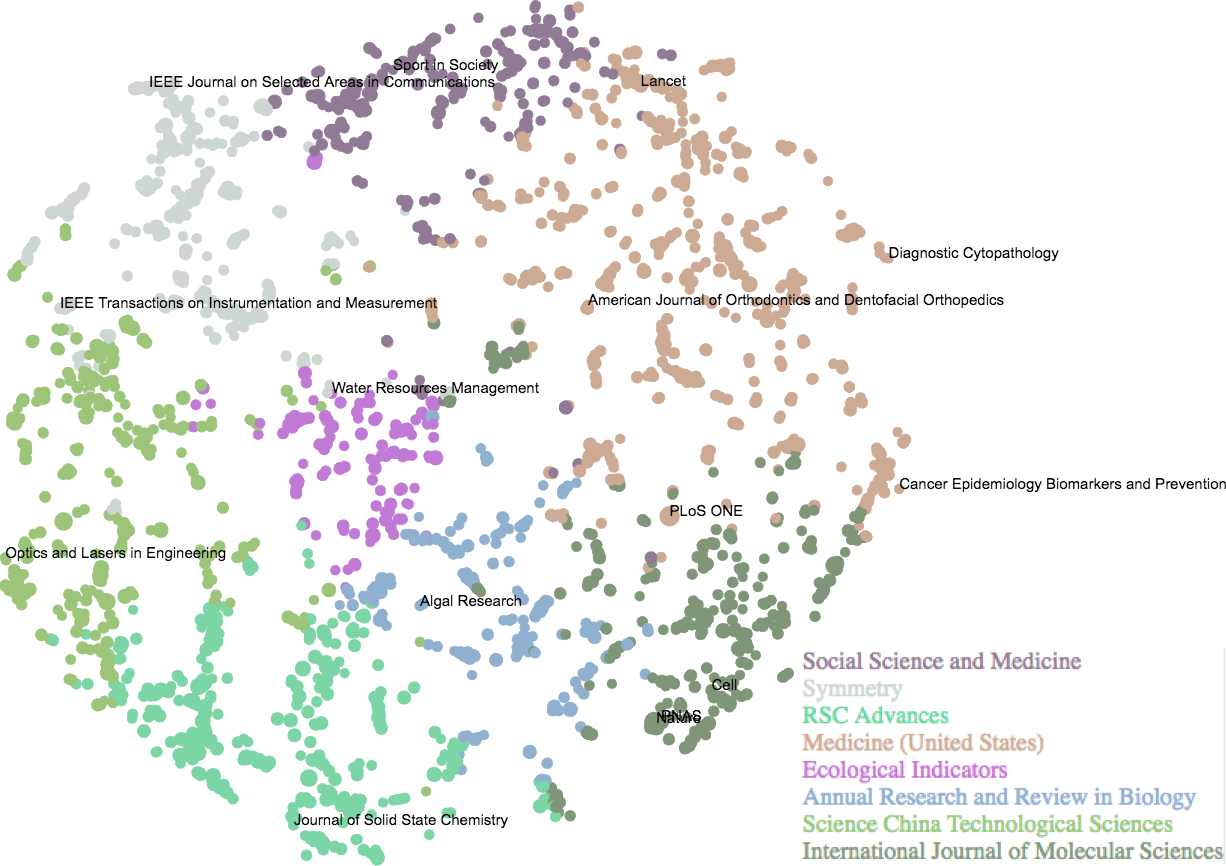
\includegraphics[height=6.5in]{Plots/Journal_Plots/Abstract_grouped}
\end{center}
\caption{Journal plot of abstract embeddings, k-means grouped}\label{figure:abstractPlotGrouped}
\end{figure}
\end{landscape}
\end{document}